\begin{frame}[parent={cmap:jabuti},hasnext=true,hasprev=true]
\frametitle{JaBUTi}
\framesubtitle{JaBUTi architecture}
\label{concept:jabuti-tools}

\begin{block:fact}{JaBUTi components}
JaBUTi architecture is comprised of several components:
\begin{itemize}
	\item \concept[definition-use-graph]{program representation},
	\concept[jabuti-visualization]{visualization}, and
	\concept[jabuti-instrumentation]{instrumentation},

	\item \concept[jabuti-test-case-execution]{test case execution} and
	\concept[jabuti-test-case-management]{management},

	\item \concept[jabuti-measurement-tool]{software measurement},
	\item \concept[jabuti-slicing-tool]{software slicing}, and
	\item and \concept[jabuti-report]{report} components.
\end{itemize}
\end{block:fact}

\begin{block:fact}{JaBUTi tools}
Those components are organized in three tools:
\begin{itemize}
	\item software \concept[coverage-analysis-tool]{coverage analysis tool},
	\item software \concept[jabuti-measurement-tool]{measurement tool},
	\item software \concept[jabuti-slicing-tool]{slicing tool}.
\end{itemize}
\end{block:fact}
\end{frame}


\begin{frame}
\frametitle{JaBUTi}
\framesubtitle{JaBUTi architecture}

\begin{block:fact}{Why so many tools?}
\begin{itemize}
	\item The coverage analysis tool comprises of most of JaBUTi's features:
	test case management, execution, instrumentation, visualization and report.
\end{itemize}
\end{block:fact}

\begin{block:fact}{Why so many tools?}
\begin{itemize}
	\item However, some guidance must be provided to define a good test
	strategy.
	\begin{itemize}
		\item The software measurement tool collects information about the
		complexity of the software under testing, which is a good hint of
		which features should be covered first.
	\end{itemize}

	\item Once detected a \concept{failure}, it must be traced to the
	\concept{fault} that triggered it.
	\begin{itemize}
		\item The slicing tool uses the execution trace of test cases to
		detect the best spots to look for faults.
	\end{itemize}
\end{itemize}
\end{block:fact}
\end{frame}


\begin{frame}[parent={cmap:jabuti},hasnext=false,hasprev=true]
\frametitle{JaBUTi}
\framesubtitle{JaBUTi architecture}

\begin{block:fact}{JaBUTi tools relationship}
\includegraphics[width=\textwidth]{resources/JaBUTi/JaBUTi-Architecture/JaBUTi-ArchitectureOverview}
\end{block:fact}

\end{frame}